% Pages 5-6 of draft v5 rebuilt (CLAUDE.md §8 item 185); merged after pages 1-4 of v5 by build.sh.
% Blue = changed or new text; red [EST] = estimated, not run.
\documentclass[conference]{IEEEtran}
\usepackage{amsmath,amssymb,graphicx,booktabs,xcolor}
\usepackage{algorithm}
\usepackage[noend]{algpseudocode}
\newcommand{\new}[1]{\textcolor{blue}{#1}}
\newcommand{\est}{\textcolor{red}{[EST]}}
\begin{document}
\setcounter{section}{4}\setcounter{figure}{3}\setcounter{equation}{5}\setcounter{algorithm}{2}
{\color{blue}% Algorithm 3 of draft v5 (CLAUDE.md §8 item 184). Only line 8 changed from v3: the re-route enters B(v, \xi)
% instead of B(v, R/2); \xi from eq. (5). Implemented as lm_tour.py plan --xi (auto = eq. (5)).
\begin{algorithm}[t]
\caption{\textcolor{blue}{\textsc{LM-Tour} (v5: discs $B(\cdot,\xi)$)}}\label{alg:lmtour}
\begin{algorithmic}[1]\small\color{blue}
\Require AI nodes with weights $w$, land graph $G$, $R$, $\rho$, $\xi$, $\theta$, $L_{\max}$
\State $A^\star \gets$ AI nodes sorted by $w$ (descending); $\mathcal{K}_1 \gets \emptyset$
\For{all $u \in A^\star$}
  \If{$d_G(u, \mathcal{K}_1) \ge R$} $\mathcal{K}_1 \gets \mathcal{K}_1 \cup \{u\}$ \EndIf
\EndFor
\State clusters $\gets$ \textsc{Grow}$(G, \mathcal{K}_1)$ \Comment{balanced Voronoi regions}
\State $\gamma \gets$ Dubins TSP-N through discs $B(u, \xi)$, $u \in \mathcal{K}_1$
\State $\mathcal{C} \gets \{v \in A^\star \setminus \mathcal{K}_1 : d(v, \text{visited}) > R/2\}$
\Repeat
  \For{all $v \in \mathcal{C}$} $\Delta L(v) \gets$ cheapest local re-route of $\gamma$ into $B(v, \xi)$ passing the window check \EndFor
  \State $v^\star \gets \arg\max_v w(v)/\Delta L(v)$
  \If{$w(v^\star)/\Delta L(v^\star) < \theta$ \textbf{or} $|\gamma| + \Delta L(v^\star) > L_{\max}$} \textbf{break} \EndIf
  \State insert $v^\star$; remove from $\mathcal{C}$ all nodes within $R/2$ of $v^\star$
\Until{$\mathcal{C} = \emptyset$}
\State \Return $\gamma$, clusters, visited nodes
\end{algorithmic}
\end{algorithm}
% Values of \xi = min(\omega, \rho, \sqrt{r^2-h^2}), \omega = 303 m, \rho = 255 m, h = 100 m (the lateral reach
% \sqrt{r^2-h^2} is the calibrated R50 of each regime): r = 1000 m: 255; r = 500 m: 255; r = 200 m: 199; r = 150 m: 99.
% Sweep of the TODO: \xi \in \{100, 175, 250\} m at every r.
}

\emph{Window check.} Every visited node must be offered a full copy of the query nearby: the stretch of
$Q\Delta \approx 2$\,km of path around its closest approach must lie within the River reach $R_Q$ of the node
($R_Q \approx 1$\,km for one window, from the saturation sweep). Candidates that break it are rejected or the stretch
is straightened.

\emph{Choosing $R$.} Kept nodes are pairwise at least $R$ apart, so discs of radius $R/2$ around them are disjoint and
$|\mathcal{K}_1| \le 4A/(\pi R^2)$ (plus a boundary term) for an area $A$. A tour through $n$ points in area $A$ is at
most $\sqrt{2nA} + O(\sqrt{A})$ [27], and Dubins turns add $O(n\rho)$, so the base tour grows as $1/R$, while River's
delivery distance grows as $R$. \new{Since $\xi \le \rho$ and $\xi \le \sqrt{r^2-h^2}$, every landmark hears the UAV
directly; we use $\xi = 255$, 255, 199 and 99\,m at $r = 1000$, 500, 200 and 150\,m, and sweep
$\xi \in \{100, 175, 250\}$\,m.}

{\color{blue}
\section{Evaluation}
\emph{Setup.} ns-3.46 with \texttt{lr-wpan} (CSMA/CA, ACK, retransmission); channel and radio as in Section~III-B
($\alpha = 3$). Three maps with 8, 12 and 15 clusters (45, 66 and 92 critical cells; capacitated $k$-medoids, at most
80 cells each). Four A2G regimes: $L_{\mathrm{obs}} = 0$, 9.0, 19.8 and 25.7\,dB in (1), calibrated on the ns-3 pass
so that $\sqrt{r^2-h^2}$ is 1015, 498, 199 and 99\,m, i.e.\ $r \approx 1000$, 500, 200 and 150\,m. Team~1 flies a
speed profile (45$^\circ$ bank, $\pm2$\,m/s$^2$), slowing to 25\,m/s or looping where a cluster would not be offered one
copy of the query (Eq.~(3)); the clue set is fountain-coded and systematic. One ns-3 run per cluster and 100 paired
draws of the matching layer per map: every scheme sees the same pass bitmaps, coded receptions and draws. Results
are exploratory ($N < 120$).

\emph{Schemes.} \emph{LM-Tour + River-FC} (proposed, Section~V). \emph{CHORD + River-FC}: the longest flyable chord
through each cluster head, bearings and visiting order chosen jointly to minimise the mean time critical cells are
left behind. \emph{FC + gather}: team~1 flies a TSP over the critical cells and circles each until its nodes hold
enough coded packets; in-cell gathering only. \emph{FC + DTSP-N}: as FC + gather, but nearby critical cells are
grouped and served from orbits chosen by a sampled Dubins TSP with neighbourhoods. \emph{Single pass, no
cooperation}: CHORD's flight; each critical cell uses only what it decodes itself. \emph{No broadcast (rotary TSP)}:
team~2 alone visits every critical cell with the full reference. \emph{Oracle}: team~2 flies straight to the target
cell.
}

\subsection{Why cooperation is needed}
Even in the favourable regime, a node 900\,m from the path receives 1,828 of 8,001 packets but its longest run is 14
packets, against $\approx$250 for one face image (Fig.~\ref{fig:a2g}). Under short range a node hears only its own
overhead segment.

\begin{figure}[t]\centering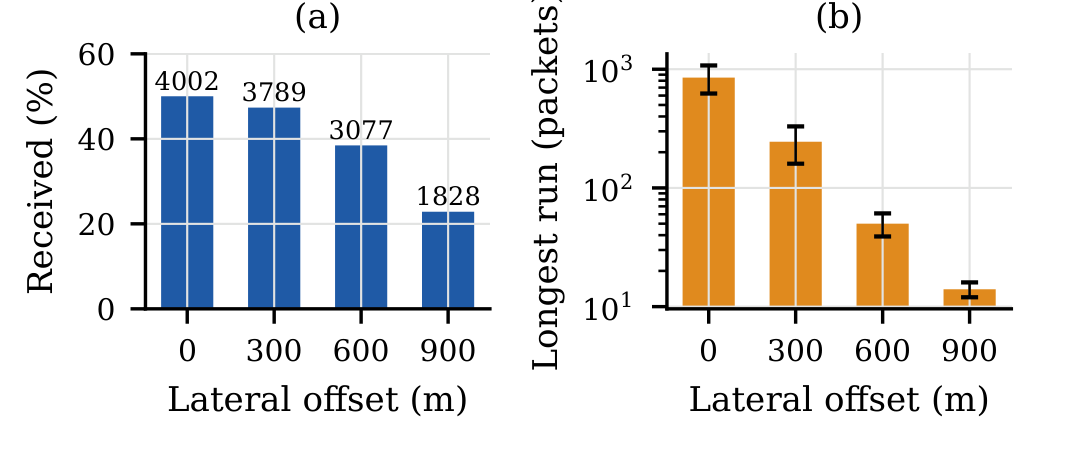
\includegraphics[width=\columnwidth]{figs/fig4-a2g-reception.png}
\caption{A2G reception at $r \approx 1$\,km (200 passes). (a) Packets received out of 8,001. (b) Longest error-free
run. Reception decays slowly with lateral offset; contiguity collapses.}\label{fig:a2g}\end{figure}

\subsection{River versus direct pulling}
With 4, 7 and 16 critical cells River uses 20--22\,\% fewer frames in 20/20 passes and finishes the last critical cell
2.7, 5.2 and 19.7\,s earlier (Fig.~\ref{fig:rvd}); with one critical cell on the SPINE the two coincide. On cluster C3
(80 cells, four critical cells) River completes the last critical cell in 37.2\,s versus 50.3\,s ($-26$\,\%) with
89.7\,k versus 102.2\,k frames ($-12$\,\%). \new{At mission level the two give the same $T^\star$ within 3\,\% in 11 of
12 settings; River never stalls, while direct pulling leaves 6 of 92 critical cells incomplete at $r = 150$\,m.}

\begin{figure}[t]\centering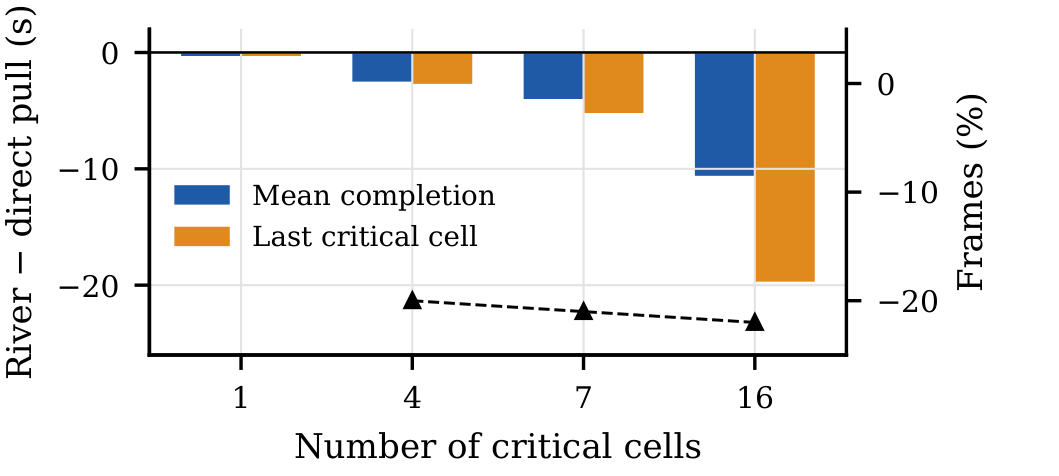
\includegraphics[width=0.85\columnwidth]{figs/fig5-river-vs-direct.png}
\caption{River minus direct pull on a 91-cell cluster (20 paired passes): completion time (bars) and MAC frames
(triangles) versus the number of critical cells.}\label{fig:rvd}\end{figure}

{\color{blue}
\begin{table}[t]\centering\caption{Critical cells complete after the pass (\%) and time from take-off to the last completion (s) versus A2G range, $K = 16$ (92 critical cells). \textcolor{red}{[EST]: estimated.}}\label{tab:complete}
\footnotesize\begin{tabular}{lcccc}\toprule
Scheme & $r=150$ & 200 & 500 & 1000\,m \\\midrule
No cooperation & 0\,\% / -- & 1\,\% / -- & 66\,\% / -- & 100\,\% / -- \\
FC + gather & 100\,\% / 7257 & 100\,\% / 6591 & 100\,\% / 2784 & 100\,\% / 1132 \\
FC + DTSP-N & 100\,\% / 6761 & 100\,\% / 5523 & 100\,\% / 2529 & 100\,\% / 1041 \\
River-FC (CHORD) & 100\,\% / 1395 & 100\,\% / 1398 & 100\,\% / 1204 & 100\,\% / 1052 \\
\textcolor{red}{River-FC + LM-Tour} & \textcolor{red}{100\,\% / 1283} & \textcolor{red}{100\,\% / 1268} & \textcolor{red}{100\,\% / 1082} & \textcolor{red}{100\,\% / 1018} \\
\bottomrule\end{tabular}\end{table}

\subsection{Robustness to the A2G regime}
Table~\ref{tab:complete}: without cooperation every critical cell completes at $r = 1$\,km, 66\,\% at 500\,m and almost
none at $r \le 200$\,m. FC-based schemes complete every critical cell only by circling: the last one completes
2.1--5.2$\times$ later than with River-FC as $r$ shrinks, whereas River-FC's completion grows by only 150--350\,s,
because River sources data from the cells under the path, which hear their own segment at any $r$.

\begin{table*}[t]\centering\color{blue}\caption{Mean mission time $T^\star$ (s), 100 paired draws, $K$ = 8 / 12 / 16 clusters. \textcolor{red}{[EST]: estimated, not run.}}\label{tab:tstar}
\setlength{\tabcolsep}{3pt}\footnotesize
\begin{tabular}{lcccc}\toprule
Scheme & $r=1000$ m & 500 & 200 & 150 \\\midrule
\textcolor{red}{LM-Tour + River-FC} & 647 / 686 / 863 & 775 / 942 / 1097 & 822 / 936 / 1143 & 810 / 942 / 1157 \\
{CHORD + River-FC} & 647 / 686 / 863 & 784 / 950 / 1107 & 876 / 975 / 1192 & 872 / 990 / 1215 \\
{FC + gather} & 660 / 815 / 949 & 1138 / 1451 / 1801 & 2285 / 3288 / 3964 & 2463 / 3460 / 4368 \\
{FC + DTSP-N} & 708 / 805 / 967 & 1078 / 1388 / 1750 & 1904 / 2482 / 3469 & 2190 / 3248 / 4468 \\
{Single pass, no cooperation} & 650 / 687 / 862 & 1379 / 2030 / 2549 & 3711 / 5277 / 6298 & 3860 / 5308 / 6358 \\
{No broadcast (rotary TSP)} & 2926 / 4168 / 5169 & 2926 / 4168 / 5169 & 2926 / 4168 / 5169 & 2926 / 4168 / 5169 \\
{Oracle} & 322 / 402 / 404 & 322 / 402 / 404 & 322 / 402 / 404 & 322 / 402 / 404 \\
\bottomrule\end{tabular}\end{table*}

\begin{figure*}[t]\centering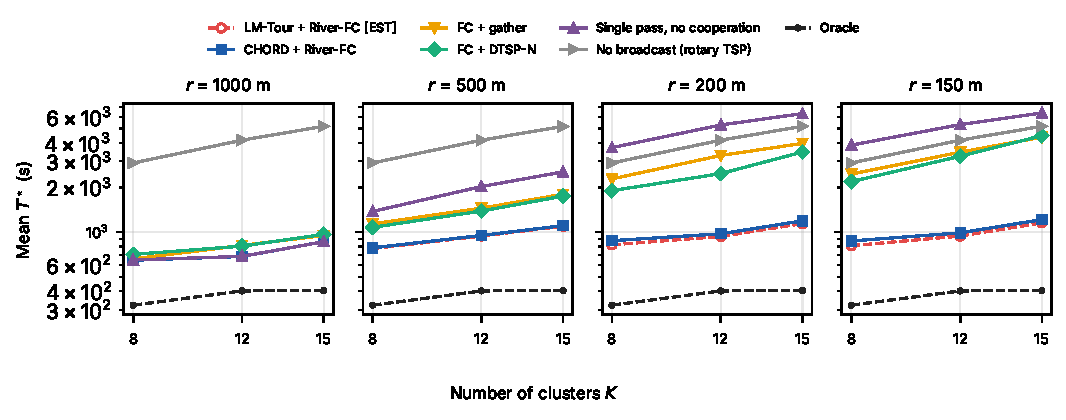
\includegraphics[width=0.9\textwidth]{figs/fig6-tstar-vs-k-4ranges.pdf}
\caption{Mean $T^\star$ versus the number of clusters, per A2G range (log scale). LM-Tour estimated \est. Oracle knows
the target cell.}\label{fig:mission}\end{figure*}

\subsection{Mission level}
Table~\ref{tab:tstar}, Fig.~\ref{fig:mission}: the single-pass architecture with River-FC is 3.3--6.0$\times$ faster
than having no broadcast phase. Against the FC baselines it is 2--15\,\% faster at $r = 1$\,km and 27--72\,\% faster at
$r \le 500$\,m, and the gap widens with $K$: CHORD's flight stays 782 / 1152 / 1415\,s at every $r$, while FC's grows
2--6$\times$. Without cooperation the same flight is 1.8--5.4$\times$ slower at $r \le 500$\,m. \est{} LM-Tour shortens
$T^\star$ by a further 1--7\,\% at $r \le 500$\,m (no change at 1\,km), by bringing the path within direct hearing of
each landmark.

\section{Conclusion}
In a single-pass UAV broadcast the flight path is the transmission schedule, so the BS can plan the ground's
cooperation before take-off. River turns this into a pre-planned, bidirectional transport that delivers the query to
the few AI-capable cameras regardless of A2G range, works with fountain coding, and pulls event frames from legacy
cameras over the same routes. Against UAV-served fountain-coded baselines the mission is 27--72\,\% faster once the
A2G range falls to 500\,m or below. \est{} LM-Tour adds 1--7\,\%. [TODO: field A2G measurements.]
}

\begin{thebibliography}{99}\footnotesize
\bibitem{} Y. Zeng, R. Zhang, T. J. Lim, ``Wireless communications with unmanned aerial vehicles: Opportunities and challenges,'' \emph{IEEE Commun. Mag.}, 2016.
\bibitem{} M. Mozaffari \emph{et al.}, ``A tutorial on UAVs for wireless networks,'' \emph{IEEE Commun. Surveys Tuts.}, 2019.
\bibitem{} Q. Wu, Y. Zeng, R. Zhang, ``Joint trajectory and communication design for multi-UAV enabled wireless networks,'' \emph{IEEE Trans. Wireless Commun.}, 2018.
\bibitem{} Y. Zeng, R. Zhang, ``Energy-efficient UAV communication with trajectory optimization,'' \emph{IEEE Trans. Wireless Commun.}, 2017.
\bibitem{} C. Zhan, Y. Zeng, R. Zhang, ``Energy-efficient data collection in UAV enabled wireless sensor network,'' \emph{IEEE Wireless Commun. Lett.}, 2018.
\bibitem{} P. Levis \emph{et al.}, ``Trickle: A self-regulating algorithm for code propagation and maintenance in wireless sensor networks,'' \emph{USENIX NSDI}, 2004.
\bibitem{} A. Shokrollahi, ``Raptor codes,'' \emph{IEEE Trans. Inf. Theory}, 2006.
\bibitem{} T. Ho \emph{et al.}, ``A random linear network coding approach to multicast,'' \emph{IEEE Trans. Inf. Theory}, 2006.
\bibitem{} H. Choset, ``Coverage of known spaces: The boustrophedon cellular decomposition,'' \emph{Auton. Robots}, 2000.
\bibitem{} E. Galceran, M. Carreras, ``A survey on coverage path planning for robotics,'' \emph{Robot. Auton. Syst.}, 2013.
\bibitem{} L. E. Dubins, ``On curves of minimal length with a constraint on average curvature\dots,'' \emph{Amer. J. Math.}, 1957.
\bibitem{} J. T. Isaacs, D. J. Klein, J. P. Hespanha, ``Algorithms for the traveling salesman problem with neighborhoods involving a Dubins vehicle,'' \emph{ACC}, 2011. [TODO: verify]
\bibitem{} W. Khawaja \emph{et al.}, ``A survey of air-to-ground propagation channel modeling for unmanned aerial vehicles,'' \emph{IEEE Commun. Surveys Tuts.}, 2019.
\bibitem{} A. Al-Hourani, S. Kandeepan, S. Lardner, ``Optimal LAP altitude for maximum coverage,'' \emph{IEEE Wireless Commun. Lett.}, 2014.
\bibitem{} F. Schroff, D. Kalenichenko, J. Philbin, ``FaceNet,'' \emph{IEEE CVPR}, 2015.
\bibitem{} J. Deng \emph{et al.}, ``ArcFace,'' \emph{IEEE/CVF CVPR}, 2019.
\bibitem{} M. Ye \emph{et al.}, ``Deep learning for person re-identification: A survey and outlook,'' \emph{IEEE TPAMI}, 2022.
\bibitem{} X. Li, A. Wu, W.-S. Zheng, ``Adversarial open-world person re-identification,'' \emph{ECCV}, 2018.
\bibitem{} Y. Shen \emph{et al.}, ``Towards backward-compatible representation learning,'' \emph{IEEE/CVF CVPR}, 2020.
\bibitem{} Y. Zeng, X. Xu, R. Zhang, ``Trajectory design for completion time minimization in UAV-enabled multicasting,'' \emph{IEEE Trans. Wireless Commun.}, 2018.
\bibitem{} J. W. Hui, D. Culler, ``The dynamic behavior of a data dissemination protocol for network programming at scale,'' \emph{ACM SenSys}, 2004.
\bibitem{} M. Luby, ``LT codes,'' \emph{IEEE FOCS}, 2002.
\bibitem{} IEEE Std 802.15.4-2020.
\bibitem{} ONVIF, ``Analytics service specification (motion detection events).'' [TODO: verify]
\bibitem{} ETSI EN 300 220-2 V3.2.1, 2018.
\bibitem{} K.-V. Nguyen \emph{et al.}, ``Efficient multi-UAV assisted data gathering schemes\dots,'' \emph{IEEE Trans. Ind. Informat.}, 2023. [TODO: volume/pages]
\bibitem{} L. Few, ``The shortest path and the shortest road through $n$ points,'' \emph{Mathematika}, 1955.
\bibitem{} 3GPP TR 38.901.
\end{thebibliography}
\end{document}
